\documentclass[10pt,twocolumn,letterpaper]{article}

\usepackage{cvpr}
\usepackage{times}
\usepackage{epsfig}
\usepackage{graphicx}
\usepackage{amsmath}
\usepackage{amssymb}
\usepackage{graphicx}
\graphicspath{{./images/}}
\usepackage{amsmath}
\usepackage{amssymb}
\usepackage{float}
\usepackage{tabularx}
\usepackage{array}
\usepackage{placeins}
\usepackage{dblfloatfix}   
\usepackage{multicol}
\usepackage{caption}
% Include other packages here, before hyperref.

% If you comment hyperref and then uncomment it, you should delete
% egpaper.aux before re-running latex.  (Or just hit 'q' on the first latex
% run, let it finish, and you should be clear).
\usepackage[breaklinks=true,bookmarks=false]{hyperref}

\cvprfinalcopy % *** Uncomment this line for the final submission

\def\cvprPaperID{****} % *** Enter the CVPR Paper ID here
\def\httilde{\mbox{\tt\raisebox{-.5ex}{\symbol{126}}}}

% Pages are numbered in submission mode, and unnumbered in camera-ready
%\ifcvprfinal\pagestyle{empty}\fi

\begin{document}

%%%%%%%%% TITLE
\title{Solving iMet: Fine-grained Multi-label Art Objects Classification with Image-Label Embeddings}

\author{Ekaterina Arkhangelskaia, Olha Sokol\\
Universit{\"a}t des Saarlandes\\
Saarbr{\"u}cken, Germany\\
{\tt\small \{s8ekarkh,s8olsoko\}@stud.uni-saarland.de }
}

\maketitle
%\thispagestyle{empty}

%%%%%%%%% ABSTRACT
\begin{abstract}
   People have been collecting art pieces even before our era. Ever since, the amount of art pieces have only been growing. With this increasing growth there is a demand in categorizing and labeling art data. Using manual labor for this purpose can be extremely expensive, therefore an automated solution is needed. Previously, there were some attempts at automated labeling of paintings \cite{Rijks}, however little research have been made in labeling different types of art, like sculpture, ceramics or applied arts. 
   In this project we attempt to perform multi-label classification task on iMet dataset. We utilize label embeddings to improve accuracy of fine-tuned ResNet18 network. Futhermore we use t-SNE algorithm to visualize learned features on artistic data. 

\end{abstract}

%%%%%%%%% BODY TEXT
\section{Introduction}
Art has always been a part of human's life. There are more than 55000 museums in the world, and due to rapid digitilizing of the world a lot of people such as researchers or other scholars would benefit from ability to quickly  navigate among all the data they contain. However, it can be time consuming and inefficient to label all the data by hand. This task motivates us to build end-to-end system to provide automatic labels for sparce and semantically different artistic data. We believe that describing finer-grained attributes from the museum-goer’s understanding, adding fine-grained attributes to aid in the visual understanding of the museum objects will enable the ability to search for visually related objects. 

\subsection{Dataset}
%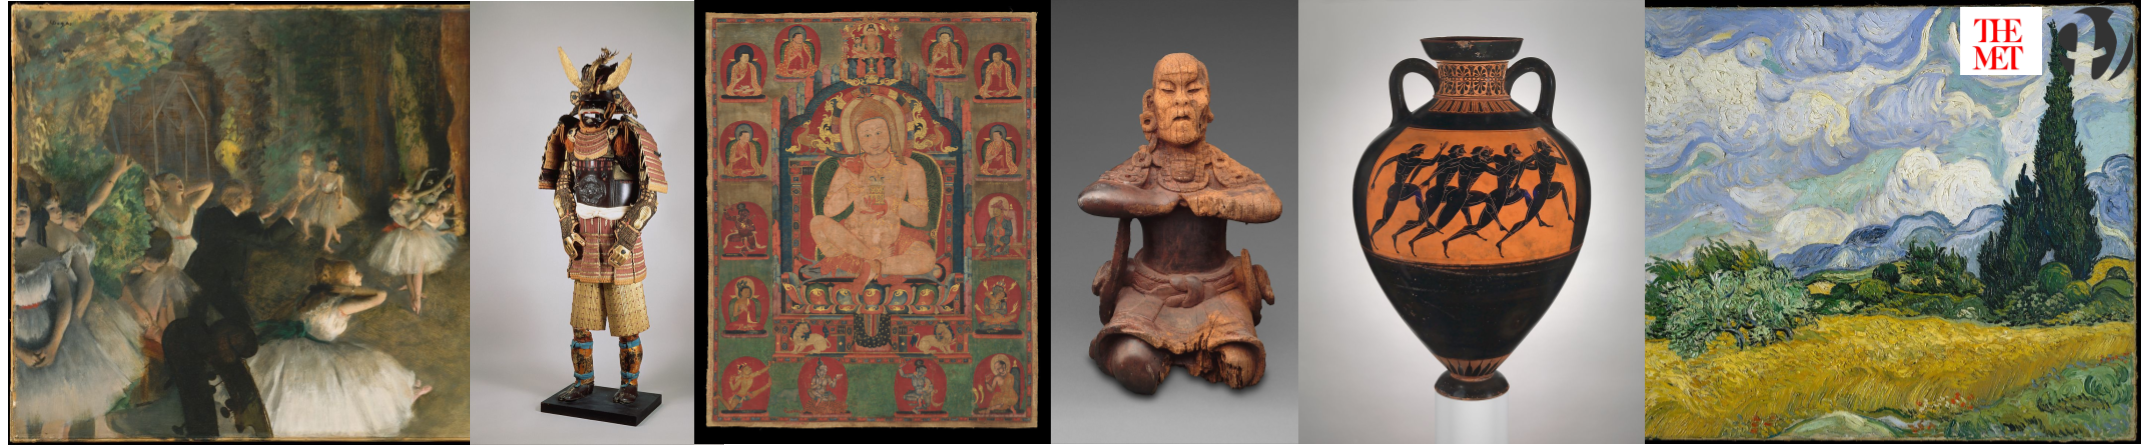
\includegraphics[width=\textwidth]{banner_imet}
\begin{figure}[h!]
\begin{center}
    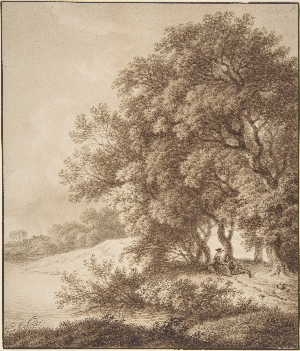
\includegraphics[width=0.25\textwidth]{sample}
\end{center}
  \caption{Sample image from dataset. Culture: central european. Tags: landscapes, lovers, men, trees, woman}
  \label{fig:imet_sample}
\end{figure}
We use iMet dataset from iMet Collection 2019 - FGVC6 challenge \cite{imet}. It is a collection of more than 109k images of different art pieces collected at Metropolitan Museum of Art in New York, also known as The Met.
Each data sample contains one image and at least one attribute label from a label set of 1103 attributes, as can bee seen on Fig \ref{fig:imet_sample}. The dimension of each image is normalized such that the shorter dimension is 300 pixels. Provided annotations are considered somewhat noisy, as they were provided by single worker without verification step. Annotations are devided into 2 categories, culture and tags, tags being related to what is “seen” or what is infered as the object’s “utility.”	

\subsection{Problem statement}
\begin{figure}[h!]
  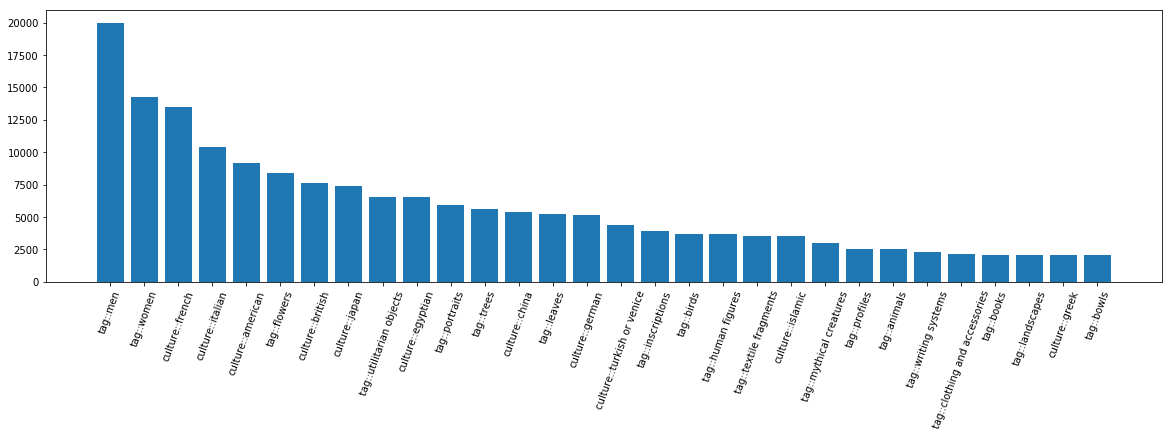
\includegraphics[width=0.5\textwidth]{labels_frequency}
  \caption{Top-30 labels by frequency}
  \label{fig:top30}
\end{figure}


As an input we use single image from iMet dataset, passing it through a neural net we want to receive a set of labels.
As we can see from Fig. \ref{fig:top30}, labels for this dataset are very unbalanced, making training conventional CNNs very challenging. To adress this issue we use labels embeddings to encourage labels close in embedding space to appear together more often.

\subsection{Related work}

There's been a lot of work in classification paintings by author, learning their artistic style  \cite{paint_class}, \cite{rec_style}, \cite{learned_style}, \cite{draw_style}, \cite{la_style}, \cite{la_style_2}, and style transfer \cite{johnson_style_transf}, \cite{huang_style_transf}, \cite{ulyaniv_stylized_img}, \cite{jie_style_transf}. However, little has been made in classification of art pieces that are not paintings. 

T. Balakrishan et al. in \cite{Rijks} tried to classify paintings of Rijksmuseum by their respective authors. To adress imbalance problem they reduces their authors set to include only top 10 artist regarding amount of paintings they produced. Then they used pretrained ResNet-18 and fine-tuned its last layer. However with such architercture they encountered accuracy drop by 0.3\% when increasing number of classes from 10 to 20.

M. Sabatelli et al. in \cite{deep_cnn_class} try to solve different classification problems on datasets similar to ours. Thy try to classify heritage art pieces from Rijksmuseum and Antwerp datasets according to their author, art style and material. To tackle this problem they use 4 architectures: VGG19 \cite{vgg}, Inception-V3 \cite{inc-v3}, Xception \cite{xception} and ResNet50 \cite{resnet50}. All of mentioned neural nets are fine-tuned with SGD in conjunction with early stopping mechanism. Categorical crossentropy loss function was used for all 3 multi-class classification problem. They also confirm idea that art features learned on Rijksmuseum dataset can be transferred on Antwerp dataset. 

Akata et al. in \cite{akata_emb} argue that attribute based image classification can be viewed as label-embedding problem. In their setup each class is embedded in the space of attribute vectors and function to optimizen is defined as 
$$f(x,w)=\underset{y \in Y}{\mathrm{argmax }}\ F(x,y;w)$$
where $w$ is model parameters and $F(x,y;w)$ measures how compatible is pair $(x,y)$ giwen $w$. They also assume that $F$ is linear in some joint feature embedding $\psi(x,y)$:
$$ F(x,y;w)=w'\psi(x,y)$$
and embedding $\psi$ can be rewritten as tensor product of image features $\theta : \mathcal{X} \rightarrow \widetilde{\mathcal{X}} = \mathbb{R}^D$ and label embedding $\varphi : \mathcal{Y} \rightarrow \widetilde{\mathcal{Y}} = \mathbb{R}^E$:
$$\psi(x,y)=\theta(x)\oplus \varphi(y). $$
To optimize $f(x,w)$ directly image classification and not only compatibility between input and output embeddings authors adapt WSABIE algorithm \cite{wsabie}. This setup proves to overcome 3 common problems existing in attribute learning. First, as mentioned before, they don't introduce intermediate problem of learning attribute classification. Then, they use training data to update label embedding by using as prior attribute embedding. Futhermore, their method can utilize other sources of additional information such as word embeddings derived from text or class hierarchies.
%-------------------------------------------------------------------------

\begin{figure*}[!ht]
	\includegraphics[width=\textwidth]{screenshot001.jpg}
	\centering
	\caption{Schemes of the two proposed network architectures}\label{fig:arch}
\end{figure*}
\section{Proposed method}
We propose a new method for imporovement of fine-grained multi-label classification tasks. Our suggestion is that by augmenting pure classification model with additional information about labels, obtained by unsuperwised learning, we would be able to improve classification results.
\par The intuition behind our method can be described as an attempt to smooth out the loss function of the multi-label classifier. That is, in the pure classifier setting the classification is regarded equally incorrect whether the predicted labels were semantically close to the ground thruth or not, as long as they are not an exact match of the true label. This makes training on the big number of labels challenging, especially since the labels in the original dataset have a wide variety of aspects they are describing and can be arbitrarily close or far in meaning across the dataset from the human standpoint. Out hypothesis is that by embedding labels into a continuous space in a way the puts classes that are close semantically close in that space and then using these vectors as an additional information for the model the learning curve of the model should be made less steep and the learning process more robust (by avoiding some local minima).
\par Our training method can be described in three stages:
\begin{enumerate}
	\item training of the Word2Vec \cite{mikolov2013efficient} model on the labels
	\item fine-tuning pretrained convolutional network on the label vectors (image-label embeddings)
	\item retraining of the convolutional network classifier on the final labels
\end{enumerate}
\par First, we use Word2Vec to project the labels into a lower-dimensional space. We define the contexts of the labels as all labels that co-occur with them in the dataset and train the embedding model to obtain the vectors for the labels at the first stage of training our classifier.
\par These vectors are then used as target values for a convolutional network based on ResNet \cite{he2015deep}. That is, we replace the last fully convolutional layer of the standard ResNet with two fully convolutional layers that are used to predict an embedding of the image's label vectors.
\par The mapping from the ResNet image features to label vectors is performed with cosine similarity loss. It is more suitable then mean squared error because the length of the embedding vector is limited (additionally, we use normalized embedding vetctors) and we mostly want to take the direction, but not the scale of the embedding into account. Additionally, we sample labels that do not belong to the given image and use the cosine similarity loss to increase idstance to their vectors.

\begin{align*}
loss(x_{img}, x_{label}) =
\begin{cases}
1-cos(x_{img}, x_{label}), \\ \text{\qquad if $x_{label}$ is a vector of some label  } \\ \text{ \qquad of the image with features $x_{img}$}\\
max(0, cos(x_{img}, x_{label})) \text{ otherwise}
\end{cases}
\end{align*}
\par We then use the resulting image embedding vector as an additional input for the classifier in two settings:
\begin{enumerate}
	\item first model (A)(Fig. \ref{fig:arch}, left) feeds the resulting embedding concatenated with ResNet features directly to the classifier
	\item second model (B)(Fig. \ref{fig:arch}, right) computes cosine similarity between image embedding and vector of every existing label and then passes these distances along with the ResNet image features to the classifier
\end{enumerate}
\par We use binary cross entropy loss for the classifier. Additionallly, we have experimented with using class weights reciprocate to the class frequency and focal loss \cite{lin2017focal} to combat class sparcity and imbalance.

\section{Experimental results}
\subsection{Label embedding examples}
While it is hard ro quantify the results of our label embedding model numerically, you can see from \cite{fig:l2v_ex} that the resulting vectors after the first stage of model training do make sense from human perspective, in that the labels that describe similar art objext are close in the embedding space.\par
Our model uses a 100-dimensional embedding size. The similar results with label embeddings were shown in spaces of lower dimension, but it was detrimental to classification results, so we have not experimented with it any further.

\begin{table*}[!t]
	\begin{center}
		\begin{tabular}{|c|c|c|c|}
			\hline
			\textbf{Label }& tag::lace & tag::food &  culture::geneva \\\hline

\textbf{\shortstack{Closest neighbors\\ with similarity}} &

\shortstack{
culture::brussels, 0.84\\
culture::antwerp, 0.82\\
culture::genoa, 0.81\\
tag::decorative designs, 0.81\\
tag::scarves, 0.80\\
tag::vestments, 0.80\\
tag::textile fragments, 0.80\\
culture::abruzzi, 0.80\\
culture::sicily, 0.78\\
tag::paisley, 0.78}&

\shortstack{
tag::servants, 0.91\\
tag::dining, 0.90\\
tag::fear, 0.88\\
tag::bedrooms, 0.88\\
tag::painting, 0.87\\
tag::family, 0.87\\
tag::anger, 0.87\\
tag::daily life, 0.86\\
tag::students, 0.86\\
tag::kitchens, 0.85}
&
\shortstack{tag::pocket watches, 0.90\\
	culture::zurich, 0.90\\
	tag::watches, 0.89\\
	culture::amsterdam, 0.82\\
	culture::swiss, 0.81\\
	culture::french or swiss, 0.80\\
	culture::strasbourg, 0.78\\
	tag::commodes, 0.77\\
	culture::st. petersburg, 0.77\\
	culture::spitalfields, 0.76}
\\
\hline
		\end{tabular}
\end{center}
\caption{Label embedding examples}
\label{fig:l2v_ex}
\end{table*}

\subsection{Image embedding examples}
Similar to label embeddings, we present examples of the closest neighbors of image embeddings after the second stage of model training. While they don't exactly match the true labels they are semantically close from the authors' perspective.
\begin{table*}[hb!]
	\begin{center}
		\begin{tabular}{|c|c|c|c|}
			\hline
			 \textbf{Test images}&	\includegraphics[width=0.25\textwidth]{japan.png} & \includegraphics[width=0.3\textwidth]{hochst.png} & \includegraphics[width=0.25\textwidth]{weapon.png} \\
			\hline\hline
			\textbf{True labels}
			&
			\shortstack{
			culture::japan\\
			tag::women\\
			tag::writing systems}
		&
		\shortstack{\\culture::german\\
			culture::hochst\\
			tag::dancers\\
			tag::dancing\\
			tag::flowers\\
			tag::women}
		&
		\shortstack{culture::italian\\
			tag::weapons}
\\		\hline\textbf{
		\shortstack{Predicted\\
			closest label\\ vectors
			with\\ similarity}}
			&
			\shortstack{\\\\
				culture::japan, 0.55\\
				tag::actors, 0.46\\
				tag::women, 0.39\\
				tag::men, 0.38\\
				tag::costumes, 0.36\\
				tag::girls, 0.34\\
				tag::mice, 0.33\\
				tag::performance, 0.29\\
				tag::fans, 0.29\\
				tag::boys, 0.28			}&
		\shortstack{
culture::german, 0.58\\
tag::sculpture, 0.44\\
culture::meissen, 0.40\\
culture::hochst, 0.40\\
culture::austrian, 0.38\\
tag::lovers, 0.37\\
tag::parrots, 0.36\\
tag::men, 0.36\\
tag::women, 0.35\\
culture::fulda, 0.34}
&		\shortstack{
tag::weapons, 0.51\\
culture::italian, 0.46\\
culture::german, 0.34\\
tag::swords, 0.30\\
tag::armors, 0.24\\
culture::french, 0.24\\
culture::flemish, 0.22\\
culture::milan, 0.22\\
tag::mythical creatures, 0.21\\
tag::firearms, 0.20}
		\\
		\hline
		\end{tabular}
	\end{center}
	\caption{Image embedding examples}
\end{table*}

\subsection{Training statistics}
You can see from the training statistics on the figures\label{fig:stat1}, \label{fig:stat2} accuracy is not a very useful measure in this task, it stays close to 1 from the start of the training because most of the examples are negative for most classes. This is why we evaluate our models with F2-score.
\par We have also experimented with combining the last two stages, but it didn't give satisfactory results, probably because training in this setting requires more subltle hyperparametrs tuning to adjust the contribution of both classification and embedding loss.
\par Training of all models took approx 5 hours each on a single Tesla P100 GPU.

\subsection{Visualization}
To provide better understanding of extracted features in final layers of our model, we use t-SNE \cite{tsne} dimentionality reduction technic. It is particularly well suited for the visualization of high-dimensional datasets, which is why we consider it suitable for our case. 
We forward a batch of images through a model and extract tensor of features of second embedding. Using t-SNE, we reduce this 100-dimentional tensor to 2-D space to plot corresponding image on a grid.
On Fig. \ref{fig:tsne} you can see that neighbouring images actually look somewhat connected, even though they don't have clear visual resembelling.

\begin{figure}[hb!]
	\begin{center}
		\begin{tabular}{|c|c|c|c|}
			\hline
\includegraphics[width=0.3\textwidth]{tsne1} &	\includegraphics[width=0.25\textwidth]{tsne2} & \includegraphics[width=0.25\textwidth]{tsne3} & \includegraphics[width=0.2\textwidth]{tsne4} \\
			\hline
	\end{tabular}
	\end{center}
	\caption{Examples of clustered images in feature space}
	\label{fig:tsne}
\end{figure}

\subsection{Evaluation}
    \begin{minipage}[b]{0.5\hsize}\centering
    	\begin{tabular}{|m{1cm}|cccc|}
		\hline
		\textbf{Model} & \textbf{F2-score} & \textbf{Recall}  & \textbf{Precision} & \textbf{Accuracy} \\ \hline \hline
		ResNet-18 & 0.4593 & 0.5314& 0.3001 & 0.9950\\ \hline
		RN-18 + emb. (A) &0.4866 & 0.5655 & 0.3125 &0.9952\\ \hline
		RN-18 + emb. (B) &\textbf{0.4929} & 0.5799 & 0.3107 &0.9950\\ \hline  \hline
		ResNet-18, focal loss & 0.4820 & 0.5624& 0.3068& 0.9951\\ \hline
		RN-18 + emb. (A), focal loss  & 0.5104 & 0.5786& 0.3469 & 0.9955\\ \hline
		RN-18 + emb. (B), focal loss & \textbf{0.5245} & 0.5844&0.3721 & 0.9955\\ \hline
	\end{tabular}
	\captionof{figure}{Model comparison}
	\label{tab:singlebest}
\end{minipage}
\par Using weighted classification has produced suboptimal results, so we do not report them here
\begin{figure*}
	\includegraphics[width=\textwidth]{clsss_emb_no_dist_focal.png}
	\centering
	\caption{Training statistics of the model A with focal loss}\label{fig:stat1}
\end{figure*}
\begin{figure*}
	\includegraphics[width=\textwidth]{clsss_emb_dist_no_focal.png}
	\centering
	\caption{Training statistics of the model B without focal loss}\label{fig:stat2}
\end{figure*}

\section{Conclusions and Future work}
In this work, we propose an improvement on a multi-label classifier for datasets with high numbers of classes. Our approach is a simple tweak over a standard model, but shows improvement of ~0.04 F2-score over regular image classifier without label embeddings.
\par
Further work would include more experiments with different convolutional networks, as well as experiments in different settings with different hyperparameters. Another approach we would look into would be separating the labels into categories and training different classifiers for each group.\par
Source code is available at https://github.com/olgasokol/iMetProject
\FloatBarrier

{\small
\bibliographystyle{ieee_fullname}
\begin{thebibliography}{9}

\bibitem{Rijks} 
Tara Balakrishan, Sarah Rosston, Emily Tang
\textit{Using CNN to Classify and Understand Artists from the Rijksmuseum}.
2017. Available at: \texttt{http://cs231n.stanford.edu/reports/2017/ pdfs/410.pdf}

\bibitem{deep_cnn_class} 
Matthia Sabatelli, Mike Kestemont, Walter Daelemans, Pierre Geurts
\textit{Deep Transfer Learning for Art Classification Problems}.
ECCV VisArt Workshop on Computer Vision for Art Analysis (September 2018, Munich GE).

\bibitem{akata_emb}
Zeynep Akata, Florent Perronnin, Zaid Harchaoui, Cordelia Schmid. 
\textit{Label-Embedding for Image Classification}
arXiv preprint arXiv:1503.08677 [cs.CV]

\bibitem{imet} 

\textit{iMet Collection}. 
 FGVC6, CVPR 2019.

\bibitem{corr_feat}
Wei-Ta Chu, Yi-Ling Wu.
\textit{Deep Correlation Features for Image Style Classification.}
ACM Multimedia 2016.

\bibitem{rec_style}
Sergey Karayev, Aaron Hertzmann, Holger Winnemöller, Aseem Agarwala, Trevor Darrell.
\textit{Recognizing Image Style.}
BMVC 2013.

\bibitem{learned_style}
Vincent Dumoulin, Jonathon Shlens, Manjunath Kudlur.
\textit{A Learned Representation For Artistic Style.}
ICLR 2016.

\bibitem{paint_class}
Wei Ren Tan, Chee Seng Chan, Hernán E. Aguirre, Kiyoshi Tanaka.
\textit{Ceci n'est pas une pipe: A deep convolutional network for fine-art paintings classification.}
IEEE International Conference on Image Processing (ICIP).

\bibitem{draw_style}
Samet Hicsonmez, Nermin Samet, Fadime Sener, Pinar Duygulu.
\textit{DRAW: Deep networks for Recognizing styles of Artists Who illustrate children's books.}
Proceedings of ICMR ’17, June 6–9, 2017, Bucharest, Romania.

\bibitem{la_style}
L. A. Gatys, A. S. Ecker, and M. Bethge.
\textit{A neural algorithm of artistic style.}
arXiv preprint arXiv:1508.06576, 2015.

\bibitem{la_style_2}
L. A. Gatys, A. S. Ecker, and M. Bethge.
\textit{Image style transfer using convolutional neural networks.}
In CVPR, 2016.

\bibitem{johnson_style_transf}
J. Johnson, A. Alahi, and L. Fei-Fei.
\textit{ Perceptual losses for real-time style transfer and super-resolution.}
In ECCV, 2016.

\bibitem{huang_style_transf}
X. Huang and S. J. Belongie.
\textit{Arbitrary style transfer in real-time with adaptive instance normalization.}
In ICCV, 2017.

\bibitem{ulyaniv_stylized_img}
D. Ulyanov, V. Lebedev, A. Vedaldi, and V. S. Lempitsky.
\textit{Texture networks: feed-forward synthesis of textures and stylized images.}
In ICML, 2016.

\bibitem{jie_style_transf}
Jie An, Haoyi Xiong, Jiebo Luo, Jun Huan, Jinwen Ma.
\textit{Fast Universal Style Transfer for Artistic and Photorealistic Rendering}
arXiv preprint arXiv:1907.03118v1, 2019

\bibitem{vgg}
Simonyan, K., Zisserman, A.
\textit{Very deep convolutional networks for large-scale image recognition.}
arXiv preprint arXiv:1409.1556 (2014)

\bibitem{inc-v3}
Szegedy, C., Vanhoucke, V., Ioffe, S., Shlens, J., Wojna, Z.
\textit{Rethinking the inception architecture for computer vision.}
In: Proceedings of the IEEE Conference on Computer Vision and Pattern Recognition. pp. 2818–2826 (2016)

\bibitem{resnet50}
Xie, S., Girshick, R., Dollár, P., Tu, Z., He, K.
\textit{Aggregated residual transformations for deep neural networks.}
In: Computer Vision and Pattern Recognition (CVPR), 2017 IEEE Conference on. pp. 5987–5995. IEEE (2017)

\bibitem{xception}
Chollet, F.
\textit{Xception: Deep learning with depthwise separable convolutions.}
arXiv preprint (2016)

\bibitem{wsabie}
J. Weston, S. Bengio, and N. Usunier. 
\textit{Large scale image annotation: Learning to rank with joint word-image embeddings.}
ECML, 2010.


\bibitem{mikolov2013efficient}
Mikolov, Tomas and Chen, Kai and Corrado, Greg and Dean, Jeffrey.
\textit{Large scale image annotation: Learning to rank with joint word-image embeddings.}
arXiv preprint arXiv:1301.3781, 2013


\bibitem{he2015deep}
He, K and Zhang, X and Ren, S and Sun, J.
\textit{Deep residual learning for image recognition. Computer Vision and Pattern Recognition (CVPR).}
2016 IEEE Conference, vol. 5, p6 


\bibitem{lin2017focal}
Lin, Tsung-Yi and Goyal, Priya and Girshick, Ross and He, Kaiming and Doll{\'a}r, Piotr.
\textit{Focal loss for dense object detection.}
Proceedings of the IEEE international conference on computer vision, 2017, pp. 2980-2988

\bibitem{tsne}
L.J.P. van der Maaten.
\textit{Accelerating t-SNE using Tree-Based Algorithms.}
Journal of Machine Learning Research 15(Oct):3221-3245, 2014.
\end{thebibliography}

\bibliography{egbib}
}

\end{document}
